% PAGES: 5
\chapter{Conclusions and Further Work}
\label{mt:c:conclusions}

The analysis of the distributed optical position correction scheme in this Master's Thesis was executed with a new simulation concept for this special case, and showed the relations between the different configurations of control and image processing. The idea of this concept came up in a preceding intensive investigation of actual researches related to \gls{UAV} realisation, stabilisation and control, and further investigations of optical possibilities of ego-motion. This review shows the necessity of automated simulation and test of marker-free visual feedback systems for the domain of \gls{UAV}. 

Additionally, investigations present a time-variant physical model for simulating each movement of the quadrocopter body. A further analysis showed how the real electronic components, like the \gls{IMU} and the actuators, provide and realise the detected and desired signals. Based on these informations, a simulation was designed and implemented using the method of \gls{MBD} and the MATLAB/Simulink tool-packages. Based on the examined results of optical models and image processing movement detection algorithms, an additionally simulation architecture was implemented, providing a flexible way to simulate different optical system behaviours.
\newpage
Beside this, the simulation was designed modular, with the aim for each component to be exchangeable, and the interface design between the modules to allow extensions for future developments. Using this simulation equipment, several camera and image processing models derived from experiments executed in similar scientific projects, used to derive test scenarios for the demonstration of the impact of different image processing parameters. These image processing test scenarios focus on the variation of different undergrounds, sample rates, image sizes and image processing algorithm specific parameters. Under consideration of different speed stimulus, the results of these test scenarios show the rotational and translational behaviour of two algorithm movement detection abilities, and their limitations related to the characteristics of the camera configurations. The distribution behaviour of the image processing system thereby was abstracted as transmission delay, which was reflected as reduced frame rate. 
 
The results of the image processing test scenarios show the weaknesses and strengths of the movement detection algorithms focussed on. Regarding the \gls{COOF} algorithm, we saw that it can detect reliable movements under high speed stress conditions, but shows increasing noise behaviour, especially with increasing frame rate, and in reduced form also with increasing image size. In comparison to that, the \gls{BMOF} algorithm showed serious speed limitations, especially in configurations with low image sizes and frame rates. Furthermore, an algorithm independent but important output signal delay behaviour, related to the image processing, was found in the small area of frame rates.
\newpage
Under consideration of the performance criteria of the designed position and body control system, optimisation experiments were executed to find the best suited parameter configuration for control. The related results show that the realistically designed not-linear physical plant cannot be optimised using linearisation analysis approaches. So the empirical optimisation approach was used with the result of the best suited parameter configuration of the control system used here. Beside this analysis, a strategy for control optimisation was derived, which can be used for further control system developments.

Combined together, and based on the results of the image processing tests and the analysis and optimisation of the control system, the quality of the position control scheme was analysed. This analysis was executed with the aim to show how the complete position correction system reacted under influence of transnational and rotational drifts, and further how it kept the hovering position.

The presented results show that it is possible to build up a distributed position correction scheme with small frame rates, but also with an adequate performance behaviour. Thereby, the test results of the image processing tests also reflected the performances of the position correction tests, and underlined them with visualisation of 3D-Trajectories of the quadrocopter flight. With recapitulating these visualisations, it was found out that the noise of the detected movements had special impact in the area of small movements like these of the hovering state. Afterwards, the speed limitation of image processing algorithms decelerated the reaction behaviour, related to the intensity of the control manoeuvre, and showed that, with decreasing speed limit a bigger flight area is needed to equalise the disturbances.
\newpage
The optical navigation is a strongly growing topic of robotic science. This work showed how the corresponding strengths of this topic can be used for \gls{UAV} stabilisation, and furthermore how the realisation can be executed systematically using simulation driven \gls{MBD}. So the optical system realisation of the \gls{HSE} quadrocopter project can base on a very useful analysis, experience and a flexible simulation structure and test facility.


\section{Further Work}

In relation to this Master's Thesis, two of the biggest projects of the Faculty of Information Technology \gls{HSE} will fuse in the future. These projects are the self-developed and maintained real time operating system \gls{DOSEK} and the introduced Quadrocopter Project. The aim thereby is to demonstrate didactically the operation of new technologies that are actually also used in the Automotive-Industry. These projects, the future developments and the exact relation of this Master's Thesis are visualised in the overview graphic 
\ref{fig:ConclusioMindstorming.pdf} \footnote{The blue circles visualise project parts which are scheduled, but not started until now}. As we can see in the black line relations, the Master's Thesis' focus was especially on the simulation of the optical position correction scheme, the control system with the corresponding \gls{HIL}-facility, and the physical model. In the near future, the optical position correction scheme realisation, presented and analysed here, will start. This process will spawn, nearly parallel, projects for communication, image processing application and camera module development.
After that, a future development will be the construction of an MATLAB/Simulink tool-kit for a simulation driven and \gls{MBD} realisable embedded system application. 
\newpage
For this purpose, already realised components of this Master's Thesis' software development can be used to realise components that can automatically generate the simulated application into C-code. This source code will be idealised for the target hardware of the quadrocopter and will execute the same time-variant characteristics of control,  image processing and so on as designed in the simulation.

For this aim, the generated application source code must be designed as a generic time or event triggered \gls{DOSEK} application. With this complete tool-chain and the code generation framework, experimental developments could be executed very fast and reliable. This will be the step to a new dimension of possibilities, which also will allow to create very complex developments like an optical autonomous control navigation. 

\begin{figure}[H]
	\centering
		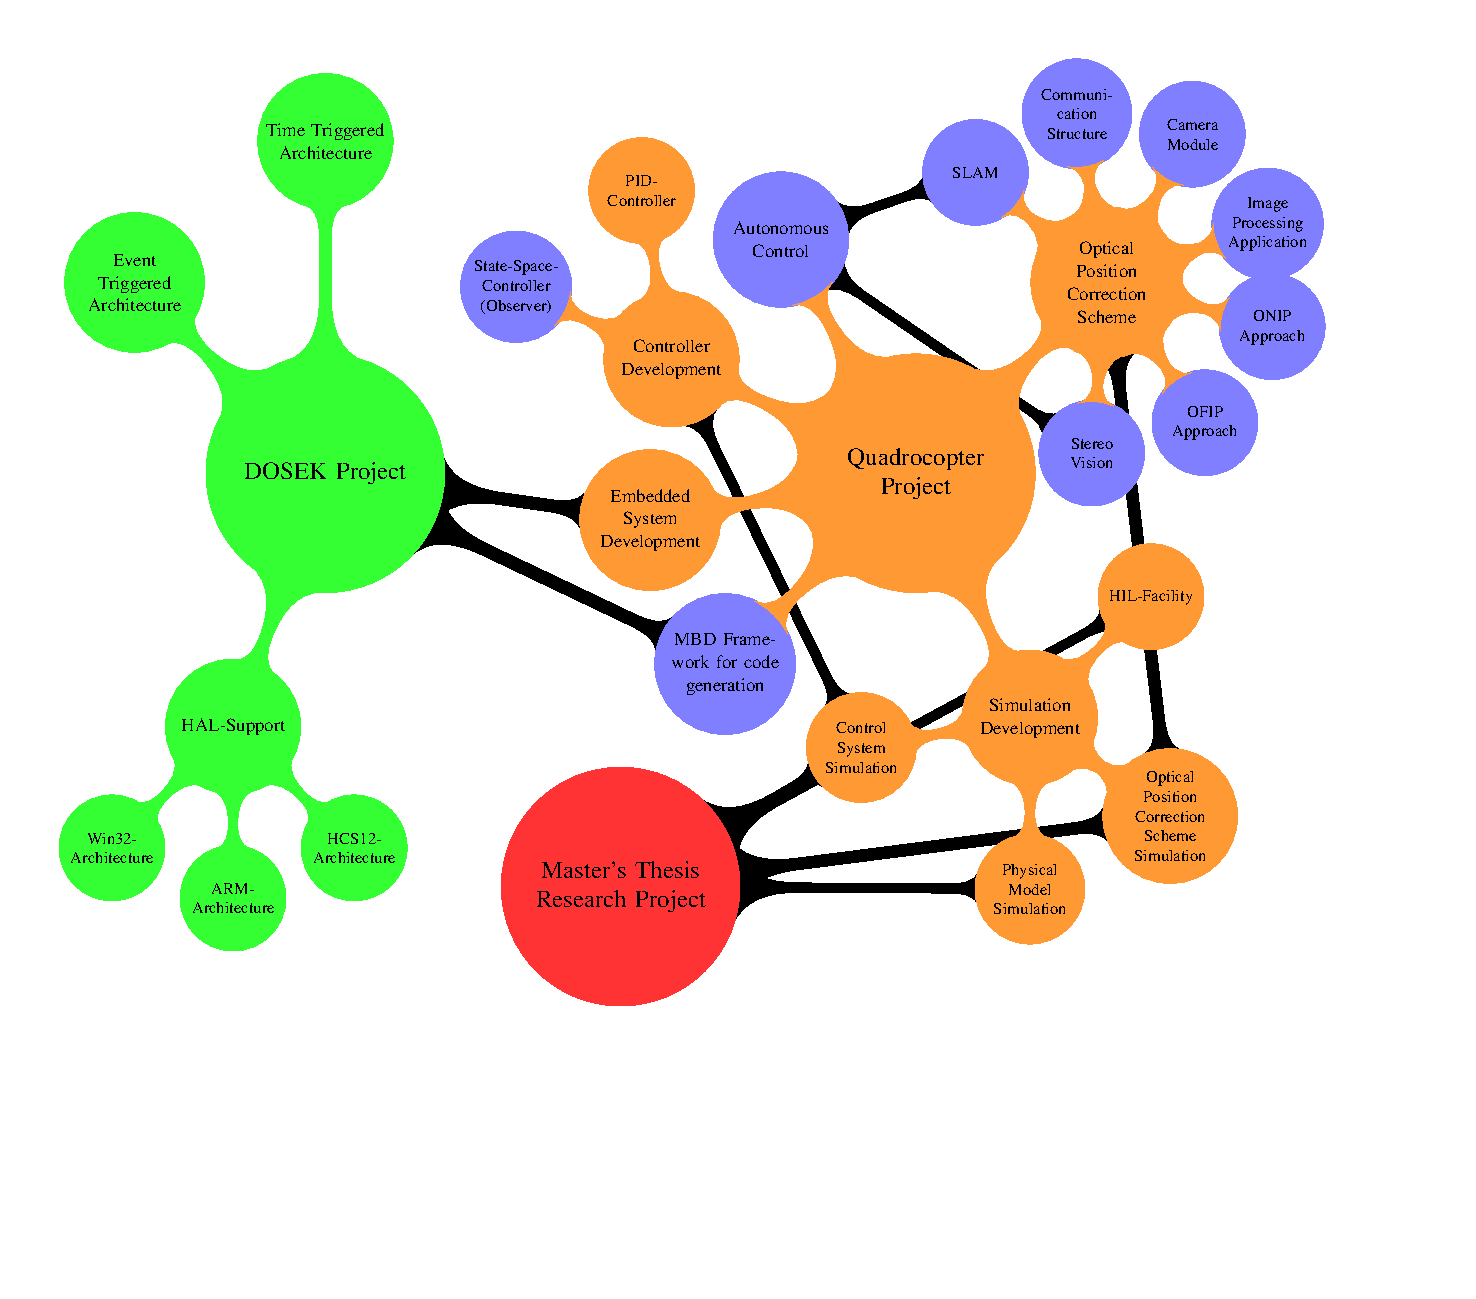
\includegraphics[width=1\textwidth]{graphic/ConclusioMindstorming.pdf}
	\caption{Overview of project relations and further work}
	\label{fig:ConclusioMindstorming.pdf}
\end{figure}